
\section{IEEE 802.15.4 protocol}

The IEEE 802.15.4 serves as a physical and MAC layers for both Zigbee and Thread 
technologies. This thesis focuses on 2.4 GHz band, because that's the frequency 
the nRF 52840 SoCs operates on. But IEEE 802.15.4 supports other bands as well 
(868.0-868.6 MHz, 902-928 MHz)\cite{802154_wikipedia}.

The protocol offers communication withing short range (approximately 10 meters) 
and the transfer rate of 250 kbit/s.

The format of an IEEE 802.15.4 frame is an important aspect to discuss. Figure \ref{fig:ieee802154_frame} presents an IEEE 802.15.4 data frame format. This kind
of frame will be used by Zigbee and Thread to send the data. The maximum length
of any 802.15.4 frame is \textbf{127} bytes. Up to 25 bytes of the frame is 
used by Frame control, Sequence number, Addressing and FCS fields, leaving up
to \textbf{102} bytes for the payload.

\begin{figure}[H]
    \centering
    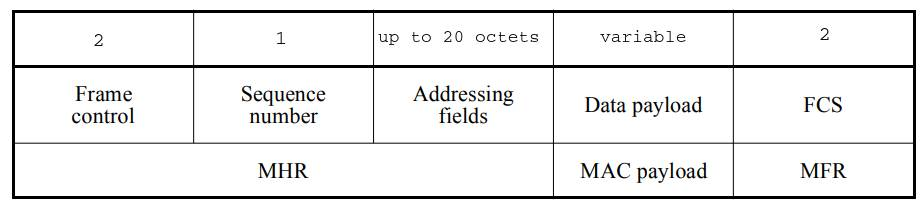
\includegraphics[scale=0.52]{images/ieee-802154-frame.jpg}
    \caption{An IEEE 802.15.4 Data Frame format, from \cite{802154_spec}.}
    \label{fig:ieee802154_frame}
\end{figure}

\section{Introduction to Zigbee}
\label{sec:IntroToZigbee}

Zigbee is a software networking protocol that provides connectivity over
an ISM radio bands. It is used mainly for home automation, medical device data collection and other domains that require low-power short range
wireless connectivity. The protocol defines a set of layers built upon IEEE 802.15.4
radio protocol, which serves as a physical and partly as a MAC 
layers\cite{ZigbeeSpecification}\cite{ZigbeeWikipedia}.

\subsection[Device roles]{Device roles\footnote{Please note that roles descriptions in this section are relevant for
centralized security model (\ref{subsec:zigbee_security}).}}

3 device roles are defined by Zigbee standard. These are: coordinator,
router and (sleepy) end device. Depending on a role, a Zigbee node carries different 
responsibilities which are especially important at a low layer of the stack.

The network coordinator is responsible for starting and forming the network. Every network has
exactly one coordinator and is assigned a randomly generated Pan ID, which is its 16 bit unique
identifier. The coordinator chooses the most optimal channel to operate on and sets up
the network to use it.
Any device eager to join the network must operate on the same channel and be let in by the coordinator. The process of joining devices that hadn't yet been the members of the 
network is called \textbf{association}.
When device is associated, it received an unique 16 bit random ID is also called short or network address.

Routers, as well as the network coordinator, participate in associating new devices into the 
network. Before they are allowed to do so, they have to be associated into the network as 
well. When a router becomes a member of the network it acts as a proxy between different devices in the network. They relay packets from one node to another. Although routers take part in associating new devices they are not allowed to
let a new devices into the network. In fact they extend coordinator's range and take over the initial
part of associating procedure (sending Beacons and Association Response packets)\cite{ZigbeeSpecification}. When a router is responsible for associating a new device
it becomes its \textbf{parent} and the new node becomes a \textbf{child} of the former. It is 
worth to mention that network coordinator behaves as a router in addition to its functions 
mentioned before.

In the Zigbee network, packets are sent asynchronously. Imagine using Zigbee for switching
the lights off or moving the blinds aside. These are clearly asynchronous signals so the 
network has to be. For that reason, routers must stay on all the time, but the nodes which
fulfil the sleepy end device role don't have to. These devices
are designed to operate on batteries and exchange little data. End devices don't route packets
and communicate with other nodes through their parent. The data from other devices are 
not sent to them directly as well. They request their parent for the data in order to get 
any. There are two types of end devices: sleepy and non sleepy. The former turn off their 
radio during periods of inactivity to lower the power consumption\cite{ZigbeeSleepyEndDevice}, whereas the
latter listens all the time.

\subsection{Security}
\label{subsec:zigbee_security}
Every Zigbee network employs the Trust 
Center device, which is usually glued together with the network coordinator, 
but can be implemented as a separate device as well. If the trust center is altogether with network 
coordinator, then a security is referred as \textit{centralized}. In the opposite case its \textit{distributed}\cite{ZigbeeSecurity}.

Trust center is an entity responsible for securing the communication within the network by
generating and distributing the keys to the nodes within the network. The communication inside the network
is secured with 2 different types of keys: network key and link key. Whilst the network key is known by every 
node in the network, the link keys are unique for all of them\cite{ZigbeeSecurity}.

It is worth to mention that in  case of Zigbee networks built with ZBOSS stack (the one used by Nordic Semiconductor), only centralized security model is supported.

\subsection{Zigbee stack layers}

The protocol is logically divided into several software layers that serve
different functions in the stack. Zigbee is aimed to run on devices with
insignificant performance, thus the stack architecture is relatively simple. The stack 
remains an IP protocol stack. However it is specifically designed to be used
altogether with IEEE 802.15.4 and the physical layer cannot be changed to another 
phy.

The Zigbee stack (presented in Fig. \ref{fig:zigbee_stack}) consists of 5 layers:
Phy, Mac, Network, APS, AF. Except the Application Framework (AF), the rest of layers is not
discussed in this thesis. For more details about them, please refer to Zigbee Specification \cite{ZigbeeSpecification}.

\begin{figure}[H]
    \centering
    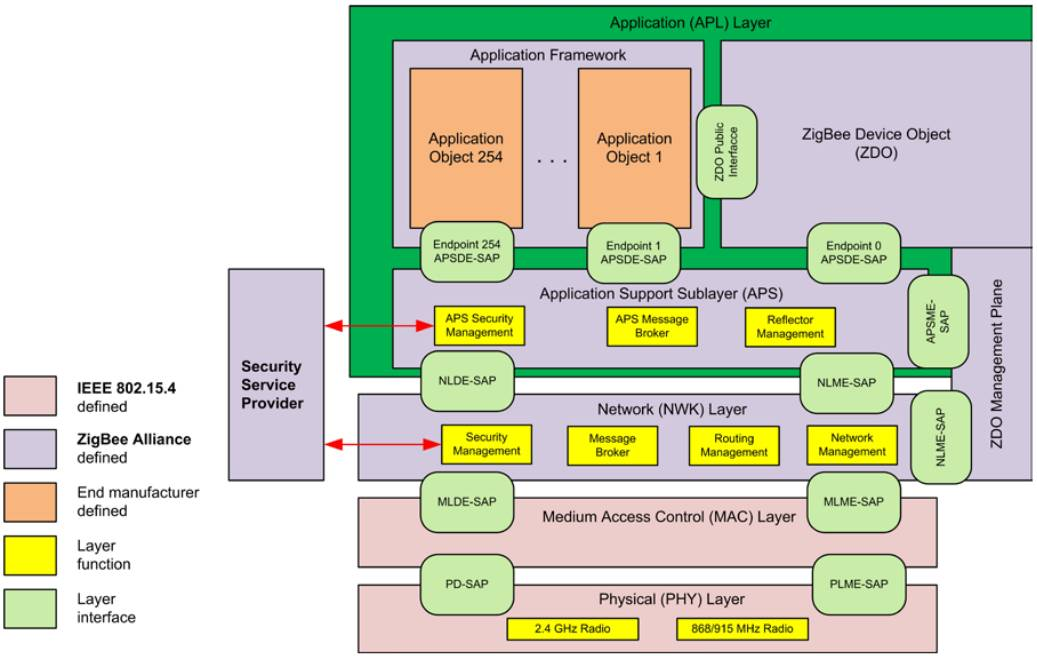
\includegraphics[scale=0.4]{images/zigbee-stack.jpg}
    \caption{Layers of the Zigbee stacks, from \cite{ZigbeeSpecification}.}
    \label{fig:zigbee_stack}
\end{figure}

\subsection*{Application Framework layer and Zigbee Cluster Library}

The top layer of the Zigbee stack - the Application Framework - is the one that users mostly interact 
with. This building block provides services for the application entities to operate. The AF exposes
256 (254 available to the user) placeholders to host different applications objects. These placeholders are called \textbf{endpoints} are given unique ids (0-255).

A specific feature of the Zigbee protocol is that applications are standardized. The set of available 
applications are specified in Zigbee Cluster Library specification. An entity representing single 
functionality of a device is called \textbf{cluster}. An application consists of a set of clusters which fulfils more complex
functionality.\cite{AddingZCLClusters}

\subsection{Zigbee frame format}

Each layer in the Zigbee stack consumes some part of the frame, decreasing the
available space for the higher layers. Just like IEEE 802.15.4 protocol's 
necessary fields occupy 25 bytes of the frame, Zigbee layers (NWK, APS, ZCL) takes
23 bytes of the remaining length. The application data must fit into \textbf{79} 
bytes long field.


\section{Introduction to Thread}

Thread is an open standard designed for low-power wireless communication  
between performance-constrained devices at lower distances (10m). Its use cases are 
similar to the ones of Zigbee (\ref{sec:IntroToZigbee}), though Thread is an
IP-based.

\section{Thread stack layers and frame format}

Although Thread stack's layers perform analogical 
function to the layers in Zigbee's stack, the protocols used on each layer are not defined by the standard.
Thread takes advantage of IEEE 802.15.4 as a MAC and physical layer as well. The network 
management and routing is held by 6LoWPAN which is a protocol enabling to run IPv6
over low-power wireless networks. It is responsible for compression and fragmentation
of IPv6 packets so they can fit into an IEEE 802.15.4 frame\cite{ThreadNordicSemi}.

On the top of 6LoWPAN, a transport layer protocols are used. In this thesis UDP protocol was utilized, but
TCP can run it as well. This layer provides a convenient interface based on sockets for 
application layer protocols. These are not covered in this thesis, because none
of them were used.

\begin{figure}[H]
    \centering
    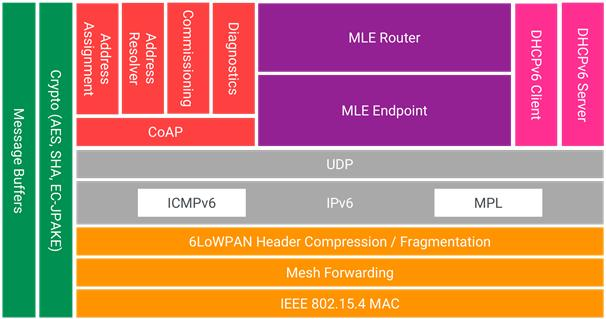
\includegraphics[scale=0.8]{images/ot_architecture.jpg}
    \caption{Thread stack architecture, from openthread.io.}
    \label{fig:thread_stack}
\end{figure}

An available payload size of an UDP packet depends on how much the IPv6 header can be compressed. 
In the project, a maximum size of \textbf{78} bytes was used. The compression of the header depends on
on a variety of factors that include: type of IPv6 addressing, 802.15.4 addressing mode and the availability of the network context\cite{ThreadUsageOf6LoWPAN}.

\section{Thread device types}

There are 4 device types in Thread\cite{ThreadStackFundamentals}. These are border routers, routers, 
router-eligible devices and sleepy end devices.

The border router is a device acting as a gateway between Thread and another adjacent IP-based network. It can, for
example, connect the Thread with WiFi or Ethernet-based networks. There is no limitation on the number of border
routers in the network.

Another device type is the router, which is responsible for providing routing services to network devices. They always 
remain on and are not allowed to sleep. Besides passing the data from one node to another, they participate
in joining and securing the communication in the network\cite{ThreadFundamentals}. 

The next type, derived from the router, is called the router-eligible end device. A node of this type acts as a router, but
due to special network topology or conditions, it can act as an end device. They have limited functions compared to
router devices. They don't provide joining or security services for other devices and are limited to forwarding
packets\cite{ThreadStackFundamentals}.

Similar to Zigbee, Thread has sleepy end devices. These can only communicate with their parents. Sleepy end devices' functions are limited to hosting and manipulating the data. They can sleep and thus save energy\cite{ThreadStackFundamentals}.

\section{Comparison of Thread and Zigbee protocols}

Although Thread and Zigbee serve similar purposes, their networking stack architectures
differ significantly. Protocol layers in Zigbee are designed especially for this stack
which can make it more robust and efficient.  Thread stack consists of a set of different networking protocols which makes
it more versatile compared to Zigbee. Being IP-based is a big advantage of Thread, 
enabling Thread devices to be available on the Internet with lower cost and effort
than Zigbee devices.

However, Thread does not specify the application layer and
any functionality and device behaviors need to be implemented. Zigbee, on the other hand, 
features ZCL and Home Automation profile which give fundamental functionalities out of the
box. These functions are sometimes sufficient when a simple product like
a light bulb or windows cover controller is developed. Zigbee runs devices with less 
performance than Thread, which is advantageous in terms of device fabrication cost. 
